\newpage
\textbf{Ejemplo 6}\\
Una persona dispone de 6.000.000 COP y como primera alternativa los puede invertir en la alternativa A que le paga un interés del 33\% nominal anual año vencido, pero solo acepta como mínimo la suma de  5.000.000 COP a un año. Como segunda alternativa puede comprar una máquina a un costo de  4.000.000 COP que le producirá ingresos mensuales por valor de  200.000 COP y al final del año podrá vender la máquina en  3.000.000 COP. Los dineros que genere la máquina podrán ser reinvertidos en la alternativa B que recibe cualquier cantidad de dinero y por cualquier tiempo siempre que no sea inferior a un mes, pero solo paga el 2\% periodo mes vencido. ¿Cuál de las dos alternativas debe tomar?
\\


\textbf{Solución.}\\

%La tabla ira centrada
\begin{center}
	\renewcommand{\arraystretch}{1.5}% Margenes de las celdas
	%Creación de la cuadricula de 3 columnas
	\begin{longtable}[H]{|c|c|c|}
		%Creamos una linea horizontal
		\hline
		%Definimos el color de la primera fila
		\rowcolor[HTML]{FFB183}
		%%%%% INICIO ASIGNACIÓN PERÍODO FOCAL %%%%%%%
		%%%%%%%%%% INICIO TITULO
		%Lo que se hace aquí es mezclar las 3 columnas en una sola
		\multicolumn{3}{|c|}{\cellcolor[HTML]{FFB183}\textbf{1. Asignación período focal}}                                                                                                                                                                                             \\ \hline
		%%%%%%%%%% FIN TITULO
		%%%%% INICIO DECLARACIÓN DE VARIABLES %%%%%%%
		\multicolumn{3}{|c|}{$pf : 0 pmv$}                                                                                                                                                                                                                                             \\ \hline

		%%%%%%%%%%% INICIO TITULO
		\rowcolor[HTML]{FFB183}
		\multicolumn{3}{|c|}{\cellcolor[HTML]{FFB183}\textbf{2. Declaración de variables}}                                                                                                                                                                                             \\ \hline
		\multicolumn{1}{|c|}{\cellcolor[HTML]{FFB183}\phantom{000}\textbf{Valores monetarios}\phantom{000}} & \multicolumn{1}{c|}{\cellcolor[HTML]{FFB183}\phantom{000}\textbf{Valores no monetarios}\phantom{000}} & \multicolumn{1}{c|}{\cellcolor[HTML]{FFB183}\textbf{Incógnitas}} \\ \hline
		%%%%%%%%%%% FIN TITULO
		%%%%%%%%%%% INICIO MATEMÁTICAS

		$ Alternativa\text{ } A $                                                                           & $ Alternativa\text{ } A  $                                                                            & $ Alternativa\text{ } A  $                                       \\
		$ P =  6\text{.}000\text{.}000\text{ } COP $                                                        & $J_x$ $=33\% naav $                                                                                   & $F_A = ?\text{ } COP$                                            \\
		$ Alternativa\text{ } B $                                                                           & $ Alternativa\text{ } B  $                                                                            & $ Alternativa\text{ } B  $                                       \\
		$ P = 4\text{.}000\text{.}000\text{ }\text{ } COP  $                                                & $ i_y = 2\%\text{ } pmv $                                                                             & $F_B = ?\text{ } COP$                                            \\
		$ F = 3\text{.}000\text{.}000\text{ }\text{ } COP $                                                 &                                                                                                       &                                                                  \\
		\hline
		%%%%%%%%%% FIN MATEMÁTICAS

		%%%%% INICIO FLUJO DE CAJA
		\rowcolor[HTML]{FFB183}
		\multicolumn{3}{|c|}{\cellcolor[HTML]{FFB183}\textbf{3. Diagrama de flujo de caja}}                                                                                                                                                                                            \\ \hline
		\multicolumn{3}{|c|}{$ $}
		%Mezclamos 3 columnas y pondremos el dibujo
		%%%%%%%%%%%%% INSERCIÓN DE LA IMAGEN
		%Deberán descargar las imágenes respectivas del drive y pegarlas en la carpeta
		%n_capitulo/img/ejemplos/1/capitulo1ejemplo1.pdf  (el /1/ es el numero del ejemplo)
		\\
		\multicolumn{3}{|c|}{$ \text{Alternativa A} $}
		\\

		\multicolumn{3}{|c|}{ 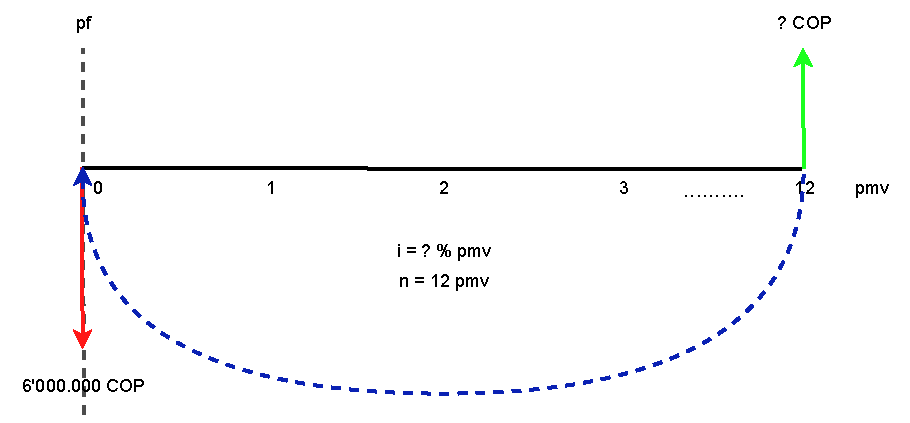
\includegraphics[scale=0.8]{ejemplos/6/Graf1Ej6Cap11.pdf} }                                                                                                                                                                                              \\
		\multicolumn{3}{|c|}{$ $}                                                                                                                                                                                                                                                      \\
		\hline
		\newpage
		\multicolumn{3}{|c|}{$ \text{Alternativa B} $}
		\\
		\multicolumn{3}{|c|}{$ $}                                                                                                                                                                                                                                                      \\
		\multicolumn{3}{|c|}{ 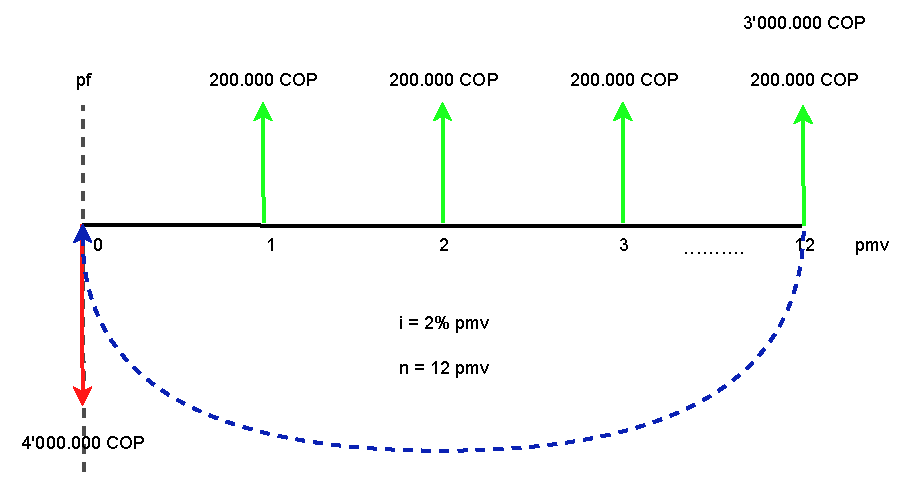
\includegraphics[scale=0.8]{ejemplos/6/Graf2Ej6Cap11.pdf} }                                                                                                                                                                                              \\
		\multicolumn{3}{|c|}{$ $}
		\\
		\multicolumn{3}{|c|}{$ \text{Reinversión} $}
		\\
		\multicolumn{3}{|c|}{$ $}                                                                                                                                                                                                                                                      \\
		\multicolumn{3}{|c|}{ 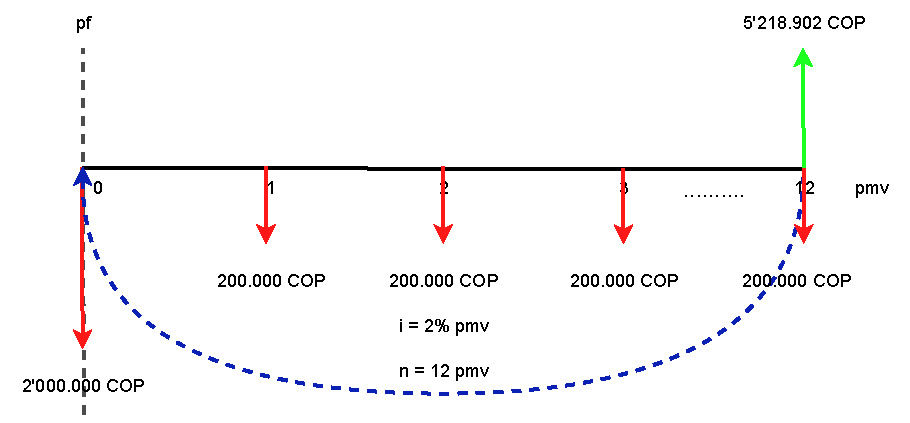
\includegraphics[scale=0.8]{ejemplos/6/Graf3Ej6Cap11.pdf} }

		\\\hline
		%%%%%%%%%%%%% FIN INSERCIÓN DE IMAGEN
		%%%%%FIN FLUJO DE CAJA



		%%%%% INICIO DECLARACIÓN FORMULAS
		%%%%%%%%%%% INICIO TITULO
		\rowcolor[HTML]{FFB183}
		\multicolumn{3}{|c|}{\cellcolor[HTML]{FFB183}\textbf{4. Declaración de fórmulas}}                                                                                                                                                                                              \\ \hline
		%%%%%%%%%%% FIN TITULO
		%%%%%%%%%%% INICIO MATEMÁTICAS
		\multicolumn{3}{|c|} {VPN =	$\sum F_{n}(1+i)^{-n}$   Valor presente neto.}                                                                                                                                                                                                     \\ \hline

		%%%%%%%%%% FIN MATEMÁTICAS
		%%%%%% INICIO DESARROLLO MATEMÁTICO
		\rowcolor[HTML]{FFB183}
		%%%%%%%%%%INICIO TITULO
		\multicolumn{3}{|c|}{\cellcolor[HTML]{FFB183}\textbf{5. Desarrollo matemático}}                                                                                                                                                                                                \\ \hline
		%%%%%%%%%% FIN TITULO
		%%%%%%%%%% INICIO MATEMÁTICAS
		\multicolumn{3}{|c|}{$ \text{La alternativa A le produce el 33\% naav} $}
		\\

		\multicolumn{3}{|c|}{$ \text{sobre el total de su capital ( 6'000.000  COP )} $}
		\\
		\multicolumn{3}{|c|}{$ \text{mientras que en la segunda alternativa podrá comprar la máquina}$}
		\\
		\multicolumn{3}{|c|}{$ \text{y le sobrarán   2'000.000  COP que podrá invertir en la alternativa B.}$}
		\\
		\multicolumn{3}{|c|}{$ \text{Y, además cada vez que la máquina le produzca un ingreso podrá} $}
		\\
		\multicolumn{3}{|c|}{$ \text{ser reinvertido en la alternativa B. Esta segunda} $}
		\\
		\multicolumn{3}{|c|}{$ \text{alternativa podría considerarse como formada por dos proyectos} $}
		\\
		\multicolumn{3}{|c|}{$ \text{así:} $}
		\\
		\multicolumn{3}{|c|}{$   2\text{.}000\text{.}000(1+0.02)^{12}\text{ } COP +   2\text{.}000\text{.}000(1+0.02)^{12}\text{ } COP ..... =    5\text{.}218\text{.}902\text{ } COP $}
		\\
		\multicolumn{3}{|c|}{$ \text{Al fusionar el primero y el segundo proyecto en uno solo se} $}
		\\
		\multicolumn{3}{|c|}{$\text{obtiene un tercer proyecto con egresos de  6'000.000  COP }$}
		\\
		\multicolumn{3}{|c|}{$\text{(   4'000.000  COP +    2'000.000  COP) y con ingresos de    8'218.902  COP}$}
		\\
		\multicolumn{3}{|c|}{$ \text{que resultan de la suma de    3'000.000  COP +  COP  5'218.902 COP} $}
		\\
		\multicolumn{3}{|c|}{$ $}
		\\
		\multicolumn{3}{|c|}{ 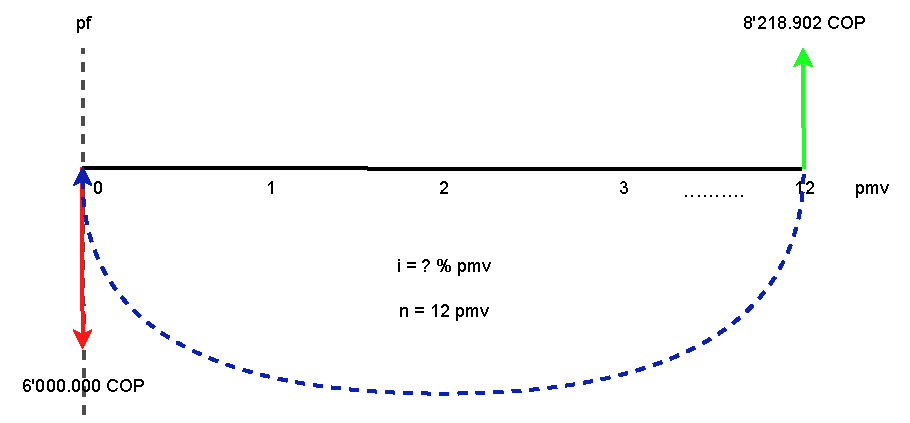
\includegraphics[scale=0.8]{ejemplos/6/Graf4Ej6Cap11.pdf} }
		\\
		\multicolumn{3}{|c|}{$ $}
		\\

		\multicolumn{3}{|c|}{$ \text{A este tercer proyecto se le puede calcular una tasa la cual}$}
		\\
		\multicolumn{3}{|c|}{$\text{viene a ser TIR+R puesto que incluye reinversión y solo usamos}$}
		\\
		\multicolumn{3}{|c|}{$\text{una tasa que es la de reinversión.}$}
		\\
		\multicolumn{3}{|c|}{$\text{La tasa de este último proyecto la calcularemos anual para }$}
		\\
		\multicolumn{3}{|c|}{$\text{compararla con la primera alternativa. }$}
		\\
		\multicolumn{3}{|c|}{$   8\text{'}218\text{.}902\text{ }\text{ } COP =   6\text{'}000\text{.}000(1 + i)^{1}\text{ } COP$}
		\\
		\hline

		%%%%%%%%%% FIN MATEMÁTICAS
		%%%%%% FIN DESARROLLO MATEMÁTICO
		%%%%%% INICIO RESPUESTA
		\rowcolor[HTML]{FFB183}
		%%%%%%%%%%INICIO TITULO
		\multicolumn{3}{|c|}{\cellcolor[HTML]{FFB183}\textbf{6. Respuesta}}                                                                                                                                                                                                            \\ \hline
		%%%%%%%%%% FIN TITULO
		%%%%%%%%%% INICIO RESPUESTA MATEMÁTICA

		\multicolumn{3}{|c|}{ \text{Se escoge la alternativa B, puesto que esta genera una rentabilidad del 36,98\% naav, mientras  }}
		\\
		\multicolumn{3}{|c|}{\text{que la primera solo genera el 33\% naav. } }
		\\
		\hline


		%%%%%%%%%% FIN MATEMÁTICAS
		%%%%%% FIN RESPUESTA
	\end{longtable}
	%Se crean dos lineas en blanco para que no quede el siguiente texto tan pegado
	%\newline \newline %USARLO SI CREES QUE ES NECESARIO
\end{center}
%%%%%%%%%%%%%%%%%%%%%%%%%%FIN EJERCICIO 1 %%%%%%%%%%%%%%%%%%%%%%%%%%%